\chapter{Metodología}
El propósito es usar métodos de simulación numérica para analizar datos que puedan ser obtenidos, lo cual, en este caso, es primordial definir cómo se implementarán.

\section{Sistema de Boyaje}

A este sistema me refiero así porque su labor será que tengamos nodos en nuestra información que nos indicarán puntos anclados que marcarán el símil de nuestros nodos de bifurcación. En este sistema no necesariamente se necesita un medio físico y podemos usar el hecho de que la interferencia de la luz provoca una gama de colores relacionable con la densidad de esa zona del medio; el ejemplo más notable lo observamos en una burbuja de jabón y agua, como puede verse en la figura 3.1:

\begin{figure}
    \centering
    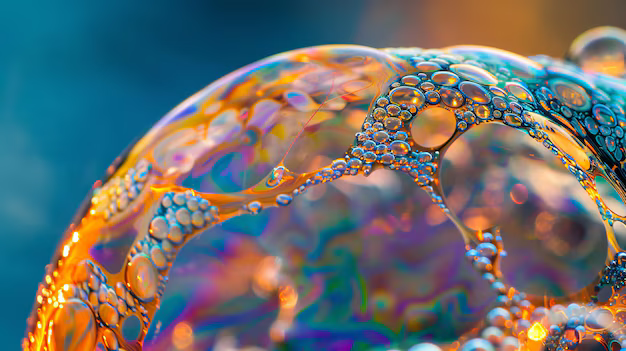
\includegraphics[width=0.5\linewidth]{Burbuja_ejemplo.png}
    \caption{Burbuja de ejemplo}
    \label{Burbuja_ejemplo}
\end{figure}

No se busca que los datos que se estudien sean de una burbuja común sino de un medio bastante controlado con una película de jabón y tentativamente se cambiaría a algún otro material, además de un fondo limpio y de color blanco, y se grabarán bajo una luz artificial blanca, en formato de video a 60 imágenes por segundo o superior en una resolución de 8 megapíxeles, esto con el fin de tener la menor cantidad de ruido en el posterior sistema de boyaje que se creará.


Principalmente los datos que se buscan obtener son una matriz de colores relacionada a la imagen de la burbuja. A este fenómeno le conocemos como interferencia de película delgada.


Volviendo a la imagen \ref{Burbuja_ejemplo} el cambio de color observado se debe principalmente a variaciones en el espesor de la película, más que a cambios en la densidad en sí. Sin embargo, la densidad del medio se relaciona de manera directa con el índice de refracción \cite{lorentz1906theory}.

La ecuación que relaciona el color visible con el espesor y las propiedades del medio es la condición para la interferencia constructiva:

\begin{equation}
2nt\cos(\theta_t) = \left(m + \frac{1}{2}\right)\lambda
\end{equation}

Donde:
\begin{itemize}
    \item $n$: Índice de refracción de la solución jabonosa que típicamente se encuentra alrededor de 1.33, pero posteriormente se realizará una muestra base y apartir de allí se dictaminará este valor.
    \item $t$: Espesor de la pared de la burbuja en ese punto específico, esto nos permitirá obtener a nuestras aristas.
    \item $\theta_t$: Ángulo de refracción de la luz dentro de la película de jabón.
    \item $m$: Un número entero ($0, 1, 2, \dots$) que representa el orden de la interferencia.
    \item $\lambda$: Longitud de onda del color observado (por ejemplo, 650 nm para el rojo o 450 nm para el azul).
\end{itemize}

Cuando la luz ambiental incide en la burbuja, una parte de la onda se refleja en la superficie exterior y otra atraviesa la primera capa, viajando por el medio fluido hasta reflejarse en la pared interior. Al salir, ambas ondas de luz se superponen y son detectadas por los microsensores de la cámara.

Debido a la gravedad y a la evaporación, el líquido de la burbuja fluye hacia abajo esto hace que la parte superior de la burbuja se vuelva cada vez más delgada y disminuye $t$ de modo que la parte inferior resulta ser más gruesa. Al cambiar $t$ en la ecuación, la longitud de onda $\lambda$ que experimenta interferencia constructiva cambia, provocando el corrimiento de colores a lo largo de la superficie.


Con base en la observación anterior, obtenemos una matriz de datos. El planteamiento fundamental consiste en utilizar la información del espesor extraída y analizada en cada pixel como la variable para definir los pesos correspondientes a los enlaces o aristas de nuestra red. Véase el siguiente ejemplo de una submatriz en una región aleatoria de la imagen, donde a cada pixel se le ha asignado un respectivo valor de espesor equivalente al grosor real de la burbuja en esa coordenada \ref{Ejemplo_submatriz}.

\begin{figure}
    \centering
    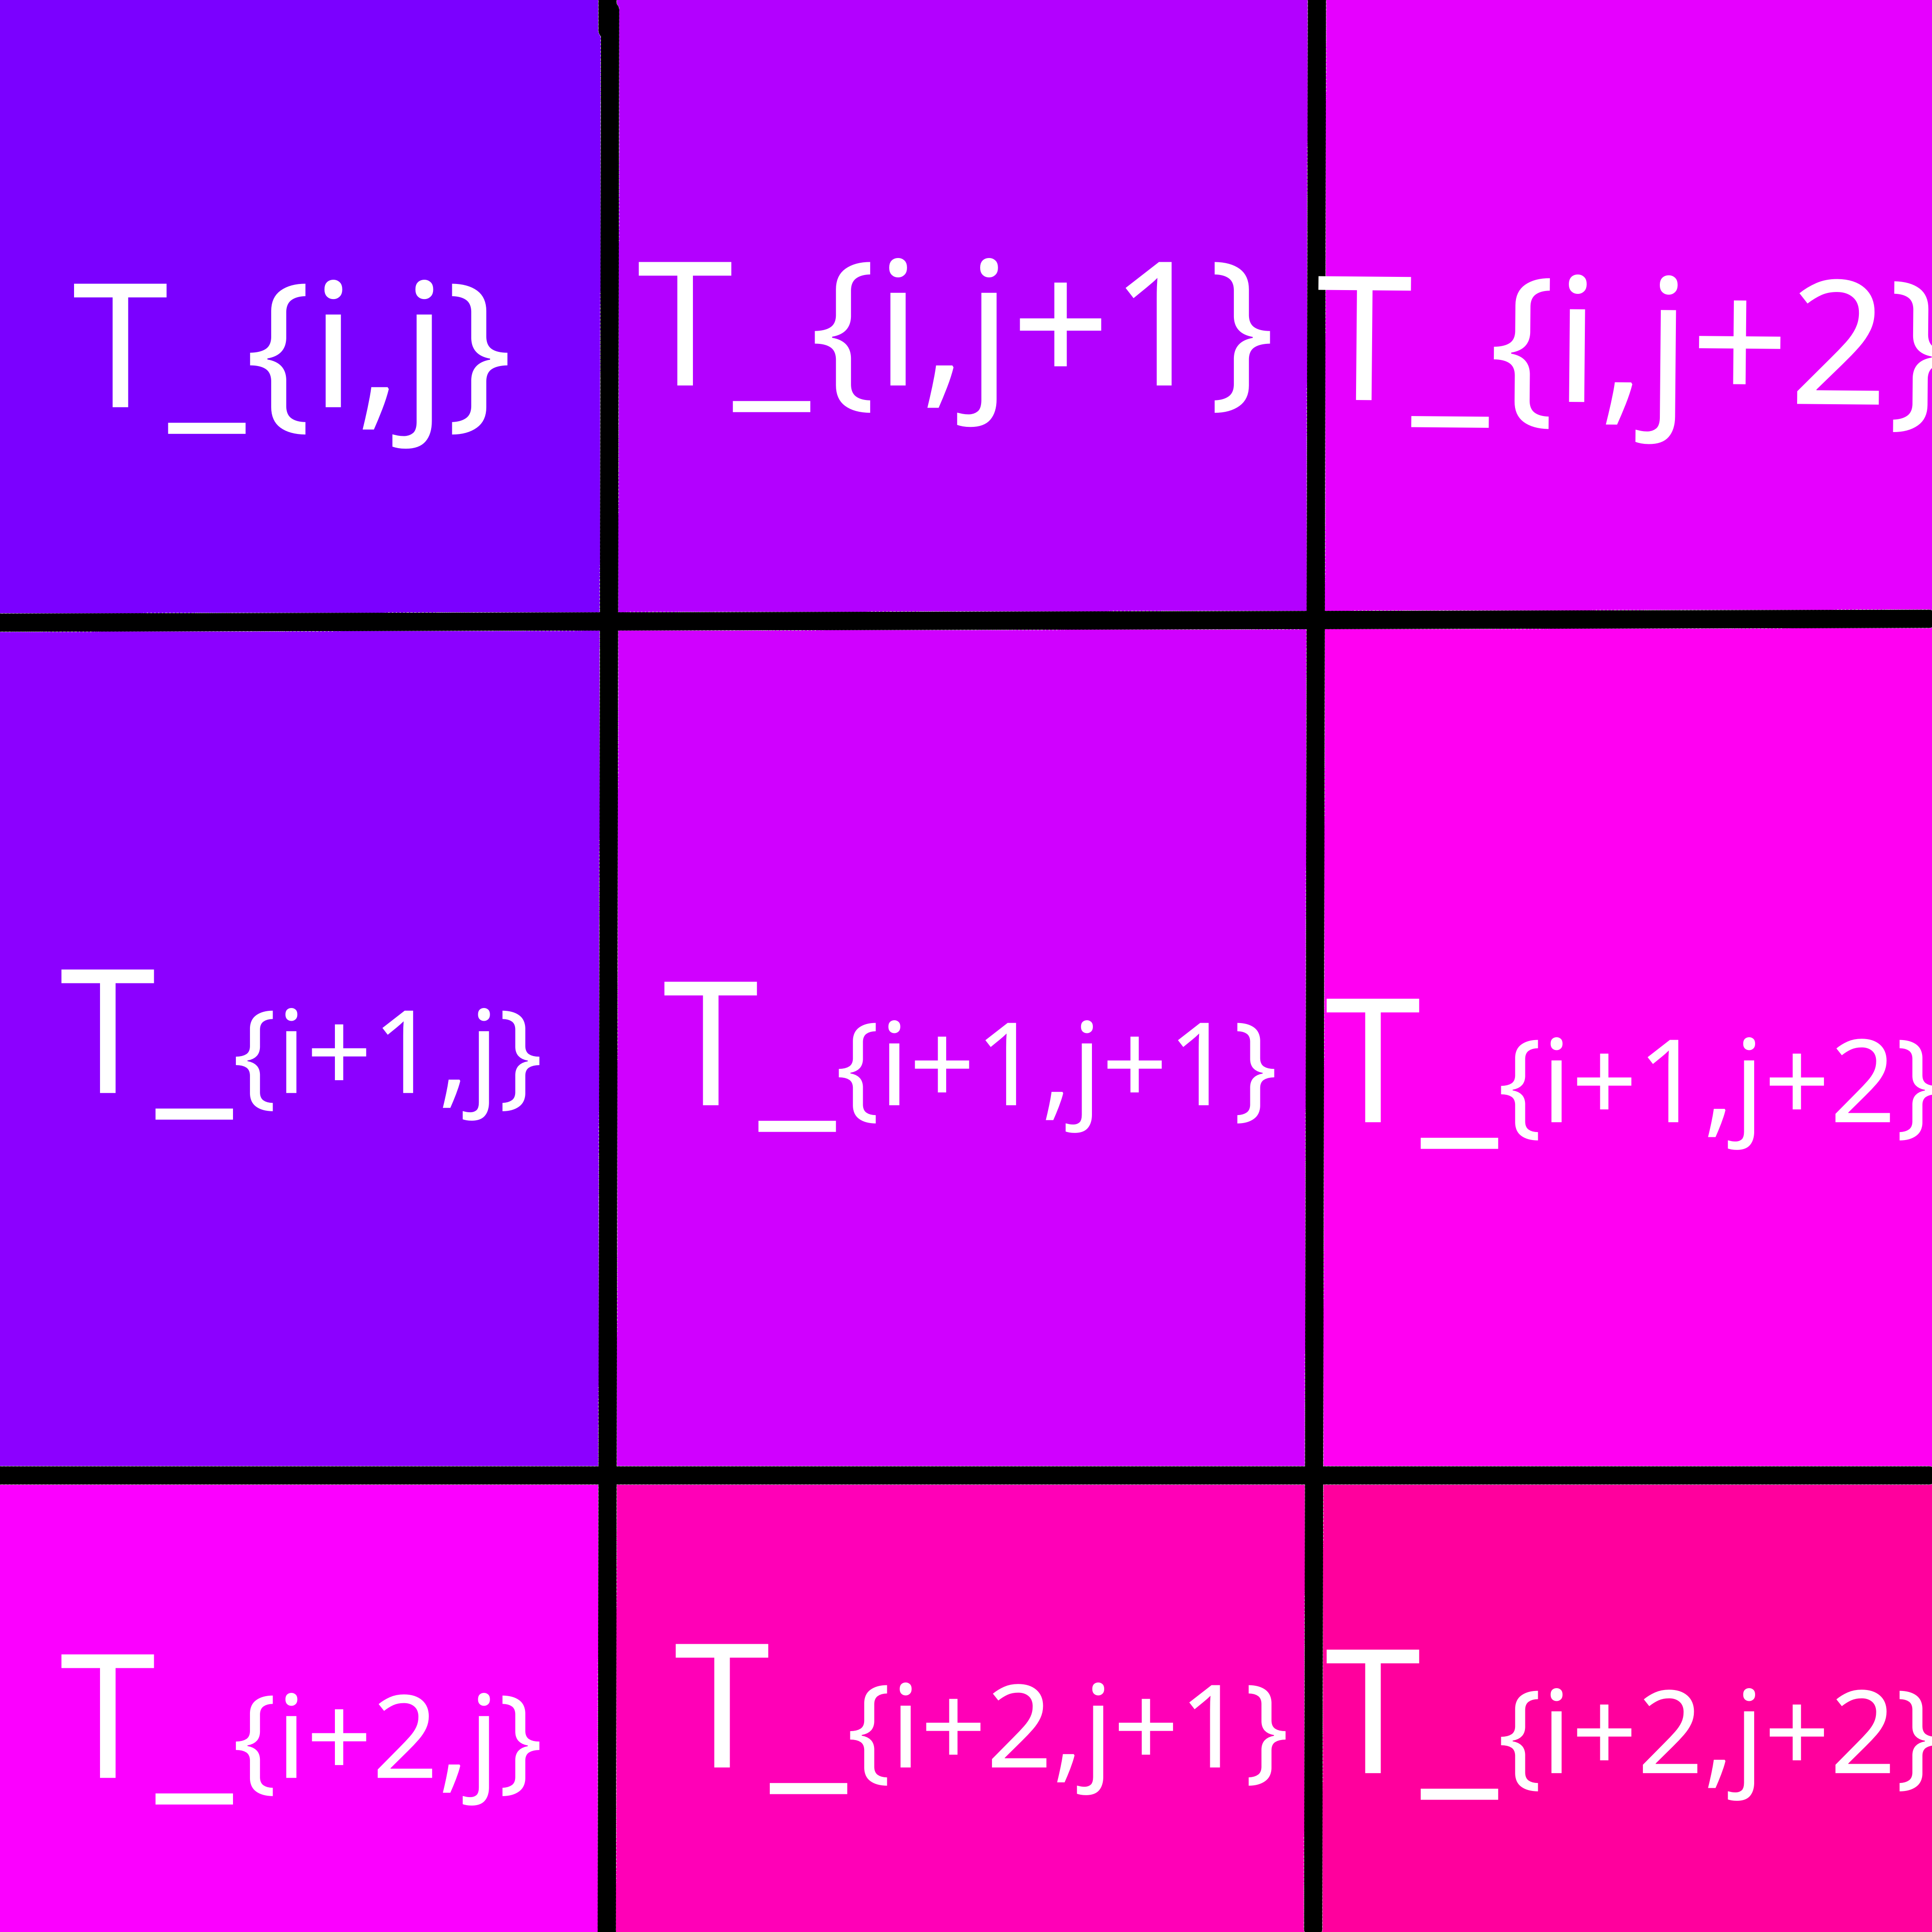
\includegraphics[width=0.5\linewidth]{Submatriz de ejemplo.png}
    \caption{Ejemplo visual donde a cada cuadrante (pixel) en la imagen le corresponde un valor continuo de espesor.}
    \label{Ejemplo_submatriz}
\end{figure}

Para modelar las trayectorias de la luz sobre este entramado, establecemos que los nodos de nuestra red no se sitúan en el interior de los píxeles, sino que se definen geométricamente justo en las esquinas de dichos píxeles. Por esta razón, como notaremos en la figura \ref{Nodos-Ejemplo}, los nodos se aprecian en las intersecciones y cruces en lugar de ubicarse en los centros, permitiendo que la información interna contenida en las facetas de los píxeles contiguos dote a las aristas de su peso estructural o costo de cruce.

\begin{figure}
    \centering
    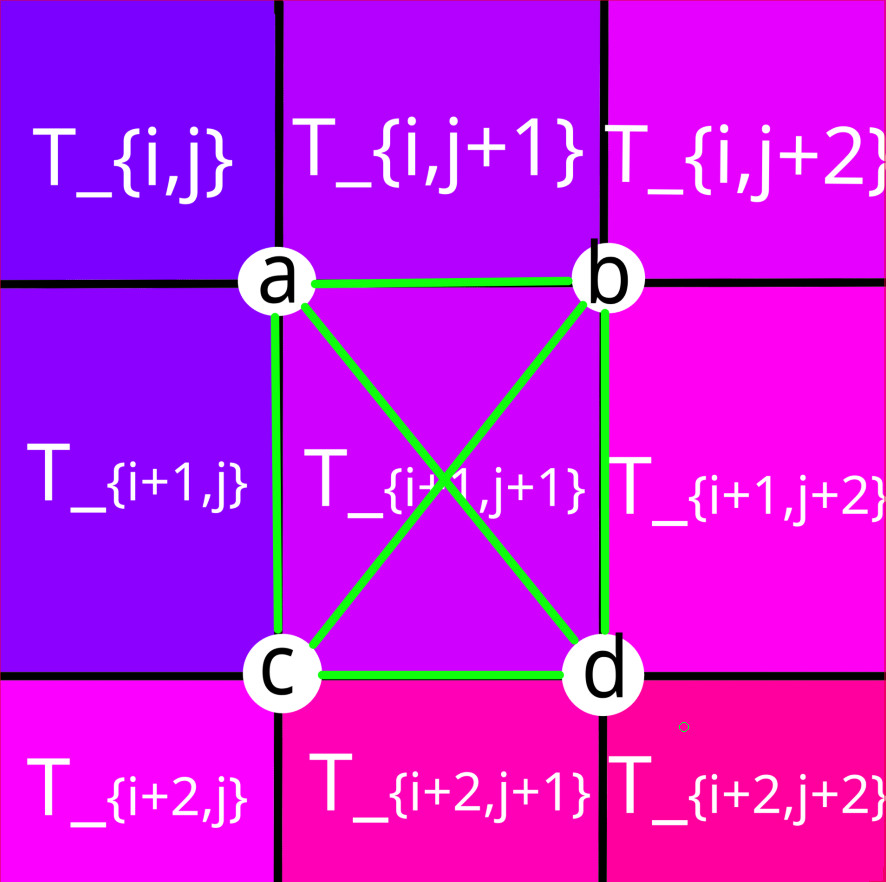
\includegraphics[width=0.5\linewidth]{Submatriz-nodos.jpg}
    \caption{Visualización de los nodos delimitados específicamente en las esquinas de un pixel bajo la retícula.}
    \label{Nodos-Ejemplo}
\end{figure}

Cabe aclarar que la subgráfica esquemática acotada por los nodos $(a,b,c,d)$ funge únicamente como un caso de exposición ilustrativa aislado para un solo elemento de retícula. Al consolidar la gráfica completa para evaluar todo el problema, este proceso se replica bidimensionalmente: en cada esquina de cada pixel se define sistemáticamente un nodo, por lo que todo pixel de la matriz aporta métricas espaciales y cada esquina en toda la imagen operará como un nodo interconector. De este modo generalizado, un nodo interno poseerá naturalmente una conectividad global de 8 vecinos adyacentes (esparcidos ortogonal y transversalmente). Durante el trayecto de un rayo, de entre estas 8 opciones posibles normalmente se contemplaría e incluiría conceptualmente al nodo antecesor inmediato; sin embargo, en el medio de la burbuja de jabón descrita y que nos atañe analizar, descartaremos fácticamente que pueda haber una retrorreflexión tan abrupta (que obligase a que el nodo sucesor sea su mismo antecesor de procedencia) dada la naturaleza refractiva continua del material.

\begin{proof}[Demostración de la ausencia de retrorreflexión en la red]

    Consideremos la trayectoria de un rayo de luz modelada como un camino definido por una secuencia de nodos $P = (v_0, v_1, \dots, v_k)$ en nuestra red. Supongamos, por contradicción, que para un nodo intermedio $v_i$, su sucesor es el mismo nodo de donde provino, es decir, $v_{i+1} = v_{i-1}$. Para que la transición por las aristas $(v_{i-1}, v_i)$ y $(v_i, v_{i+1})$ sea válida y consecutiva de esta forma, el rayo debería experimentar un cambio de dirección de $180^\circ$ exactamente en el nodo $v_i$.
    
    Sin embargo, por la naturaleza física del medio continuo transparente que estamos modelando para este caso,a posterior manejaremos a los obstáculos de una forma distinta, las perturbaciones en la densidad y el índice de refracción efectivo son paulatinas. Según la óptica de rayos en medios continuos con gradientes suaves de refracción, la curvatura y desviación del momento de la luz cambian el ángulo de propagación en cantidades pequeñas $\delta \theta$. Un retorno abrupto requeriría chocar contra una barrera opaca o un salto discontinuo gigantesco del índice de refracción, lo cual no existe en el fluido en reposo. Por ende, es físicamente imposible que un rayo se refleje sobre su misma trayectoria hacia el nodo anterior, demostrando formalmente que en nuestra topología de red se cumple siempre que $v_{i+1} \neq v_{i-1}$.

\end{proof}

Por lo mismo en caso de que se encuentra un dato que indique reflexión total se asume que será por la cuestión de pixeles muertos o ruido en la imagen y se completará la información calculando según la media de la información de los vecinos para tener una gráfica completa.

Así podemos definir los arcos, los cuales quedarían sin dirección entre cada nodo con cada uno de sus vecinos. En el ejemplo, el arco de $(a,d)$ y el arco $(b,c)$ tendrían un peso igual, y por otro lado el arco $(a,b)$ tomaría como valor la media entre $T_{i,j+1}$ y $T_{i+1,j+1}$; concretamente se espera que en su mayoría los rayos sigan una trayectoria prácticamente recta, pero algunos cuantos obtendrán una desviación que será gradual en algún nodo.

\begin{proof}[Demostración de igualdad de pesos en arcos simétricos]
    En el primer caso propuesto, afirmamos trivialmente que el arco $(a,d)$ y el arco $(b,c)$ tendrían un peso igual. Conviene recordar que el espesor de la película de jabón varía de manera preponderante en el eje vertical debido, como ya se mencionó, a los efectos de la gravedad que drenan el fluido hacia la base. Esto dota al fenómeno de una simetría traslacional local horizontal; en un mismo nivel de altura o renglón, los valores de espesor son prácticamente uniformes. Por lo tanto, si la luz transita por vías homólogas (los trayectos a una misma altitud o desplazamientos idénticos entre nodos), los cambios en la densidad son equiparables. La invariancia horizontal dictamina entonces que los costos o transiciones de dichos arcos experimentarán el mismo comportamiento constante, logrando así $w(a,d) = w(b,c)$.
\end{proof}

\begin{proof}[Demostración de la asignación del peso del arco mediante el Teorema del Valor Medio]
    Para la segunda afirmación, se debe fundamentar por qué un arco visto como la conectividad entre un par de nodos, por ejemplo $(a,b)$ debe definirse aritméticamente como la media entre sus mediciones extremas e.g. $T_{i,j+1}$ y $T_{i+1,j+1}$ Si analizamos al arco como el camino unidimensional continuo de longitud $L$ recorrido por la luz su espesor afecta a toda la propagación por el arco equivale al promedio de la función del grosor para ese tramo curvo contínuo $s$ esto se puede modelar integralmente así:
    \[ \langle T \rangle = \frac{1}{L} \int_{0}^{L} T(s) \, ds \]
    Ahora través del teorema del valior medio, se establece que para esta función continua en un intervalo cerrado existirá siempre un punto intermedio $c \in (0, L)$ tal que la función evaluada en él devuelva exactamente nuestro promedio analizado: $T(c) = \langle T \rangle$.
    
    Puesto que se define una red matricial para este problema y los pasos diminutos $L$ relativos al tamaño macroscópico de la película y sobre un sistema cuya evolución fluida no presenta discontinuidades abruptas, resulta válido ensayar una aproximación lineal de primer orden para los gradientes en $T(s)$. 
    
    Ahora, el área bajo la curva se conforma por un trapezoide con bases correspondientes a los puntos de muestreo adyacentes. Explotando las propiedades geométricas de este, el TVM recae en establecer a dicho punto $c$ en el centro de masa de la función, el cual coincide obligatoriamente de forma exacta con la media aritmética de ambos extremos del tramo:
    \[ \langle T \rangle \approx \frac{T_{inicio} + T_{fin}}{2} \]
    
    Por lo tanto es válido establecer el peso de un enlace como el promedio simple de sus enlaces adyacentes.
\end{proof}

El punto es que tengamos una red suficientemente densa en sus nodos de referencias o boyas, como para tener una información suficientemente congruente a la realidad del fenómeno que se observa.

\section{Algoritmo Computacional para el Trazado de Luz}

Para simular la propagación de la luz a través de la red descrita anteriormente, es necesario definir un algoritmo que recupere y explore las posibles trayectorias calculadas con las restricciones dadas. 

\subsection{Fundamento Físico y Matemático}
En el modelo de red reticular sobre la película de jabón, cada nodo actúa como un punto de evaluación espacial, y los pesos de las aristas determinan el costo óptico dictado por las variaciones del grosor continuo $T$ e índice de refracción. Así, el trayecto de propagación principal puede aproximarse encontrando el camino de costo mínimo desde uno o múltiples nodos fuente hacia el resto del entramado.

Dado que todos los valores de grosor extraidos y asignados a los arcos son rigurosamente positivos y calculables según las propiedades ópticas demostradas previamente, se usará el Algoritmo de Dijkstra para dar solución en nuestro grafo. No obstante, para corresponderse con la física del problema y respetar la condición de imposibilidad de retrorreflexión local directa así el código convencional se adapta: en la etapa donde cada vértice explora a sus vecinos adyacentes, el flujo excluye intencionalmente examinar en retroceso hacia el mismo nodo del que acaba de derivarse

\subsection{Pseudocódigo Transversal}

\begin{algorithm}[H]
\caption{Cálculo computacional de trayectorias en flujo ramificado}
\begin{algorithmic}[1]
\Require Grafo $G = (V, E)$, matriz de nodos y sus aristas. Función de peso $w(u,v) > 0$ derivada del grosor visual del jabón. Conjunto fuente de luz $S$. Distancias iniciales estructuradas al infinito.
\Ensure Rutas continuas óptimas para los rayos virtuales simulados con matrices de distancias y predecesores para reconstruir toda la red del medio.

\State $dist[v] \gets \infty$ para todo $v \in V$
\State $dist[s] \gets 0$ para todo $s \in S$
\State $prev[v] \gets$ NULO para todo $v \in V$ 
\State Insertar todos los nodos $V$ en una Cola de Prioridad $CP$ usando $dist$

\While{$CP$ no esté vacía}
    \State $u \gets$ extraer nodo en $CP$ con el valor mínimo actual en $dist[u]$
    \State RemoveMOS a $u$ de $CP$
    
    \If{$dist[u] == \infty$}
        \State \textsc{break} \Comment{Los sub-grafos remanentes ya no logran ser iluminados}
    \EndIf

    \For{cada nodo $v$ colindante a $u$ (vecindad máxima 8-adyacente)}
        \If{$v == prev[u]$}
            \State \textsc{continue} \Comment{Restricción física prohibitiva de retrorreflexión contigua}
        \EndIf
        
        \State $costo\_cruzado \gets w(u, v)$ \Comment{Adscrito gracias al Teorema del Valor Medio}
        \State $paso\_acumulado \gets dist[u] + costo\_cruzado$
        
        \If{$paso\_acumulado < dist[v]$}
            \State $dist[v] \gets paso\_acumulado$
            \State $prev[v] \gets u$ \Comment{Conservación fiel de la direccionalidad del rayo}
            \State Actualizar y cambiar la prioridad de $v$ en $CP$
        \EndIf
    \EndFor
\EndWhile
\State \Return Relevamiento paramétrico de árboles a lo largo de $prev[v]$ \Comment{Bifurcaciones listadas}
\end{algorithmic}
\label{alg:SimulacionFlujo}
\end{algorithm}

\subsection{Contabilidad de Complejidad Espacial y Computacional}

Las viabilidad del simuladores esta drasticamente condicionadas por las eficiencia de las implementaciónes. Al lidiar con imajenes densa grabadas para el laboratorio, cada fotograma procesado podrian tener dimensiónes desde 4 asta 8 megapixeles es decir entre 4 y 8 millones de nodo $V$.

\subsubsection{Tiempo Computacional:}
Si se ejecuta construyendo la cola de prioridad $CP$ por medio de un montículo binario el tiempo invertido en la extracción del vértice mínimo es del orden de $O(\log N)$. Y la rebaja secuencial de la distancia de los vínculos incidentes añade de igual forma ciclos del orden $O(\log N)$, siendo siempre $N = |V|$ el total de vértices instanciados, y $E = |E|$ el umbral absoluto de aristas o arcos conformables.
A lo extenso de la iteración principal cada nodo se procesa unívocamente una vez y todo arco vecinal afín es calibrado, llevando a un registro máximo acotado como:
\[\text{Complejidad} = O((N + E) \log N) \]
Recalcando las asunciones establecidas por la topología de la burbuja, el entramado asigna para todo píxel u holgura interna una conectividad delimitada de $8$ conductos por esquina. Esto garantiza algebraicamente que la cantidad máxima de fronteras evaluables será proporcionalmente un factor constante del número de puntos nodales evaluados $(E \approx 8N)$, con lo cual reducimos el margen asintótico en su cota superior, dando un resultado temporal de $O(N \log N)$. Este logro nos afirma que el algoritmo es escalable y manejable en un margen muy favorable dado el enorme grado de escala del proyecto, posibilitando analizar múltiples cuadros de video para medir los cambios de trayectoria con el tiempo. El uso, de ser menester, de estructuras avanzadas como el Montículo de Fibonacci reduciría la asintótica hasta teóricamente $O(E + N \log N)$, mejorando aún en fracciones la carga principal.

\subsubsection{Complejidad de Espacio:}
La resolución analítica exige conservar copias inmersas del entramado posicionado; para el dimensionamiento del arreglo se definen tensores bidimensionales proporcionales a lo evaluable; es necesario guardar un valor de rastreo temporal (`dist`) en punto flotante por pixel, y registrar su ruta de derivación (`prev`) en una cuadrícula simétrica paralela. Conociendo que el grafo se representa en su forma matricial abstracta (o en variables locales alocadas como mapa), la densidad en la RAM subyace bajo una estricta limitación lineal correlacionada y regida intrínsecamente del factor nodular. Entonces la contabilidad del almacenamiento dicta que la complejidad en la huella de memoria sea de
\[ O(N) \]


Finalmente se analizarán las siguientes propiedades:
\begin{itemize}
    \item Distribución de grado de los nodos de bifurcación
    \item Robustez del flujo ante cambios en la varianza de la densidad del medio
    \item Identificación de caminos críticos o puentes en la red de luz
\end{itemize}




